%% refer q31.tex

\chapter{Proposed System} 

\section{System Working}

 \hspace{0.5cm}Ultrasonic sensor is connected to the Arduino which will act as an input. The heart of our system is an ultrasonic sensor. It serves the purpose of detecting the hands of the user for dispensing the sanitizer liquid.
  
 Bidirectional visitor counter with alert system is the second stage of the system. It uses an IR sensor to sense the entry and exit of people. If a person tries to enter the premises without sanitizing their hands, a buzzer will beep continuously until the sanitizer is used again. Also a message is sent to the registered mobile number with an alert message, "Alert! Entry detected without sanitization". This feature keeps the record of the number of people present inside the premises by displaying it on an LCD display which is present at the entrance and also alerts the security personnel by making a continuous beep sound if someone tries to enter without using the sanitizer.
 
 The third stage is automatic refilling of sanitizer bottle. The sanitizer bottle refills automatically from the tank which is placed behind the system, as soon as the sanitizer level drops below a certain level in the sanitizer bottle. This detection is again done through an ultrasonic sensor and a pump is used for refilling the sanitizer bottle.


\newpage
\section{Prototype Design}
\begin{figure}[h]
		\centering
	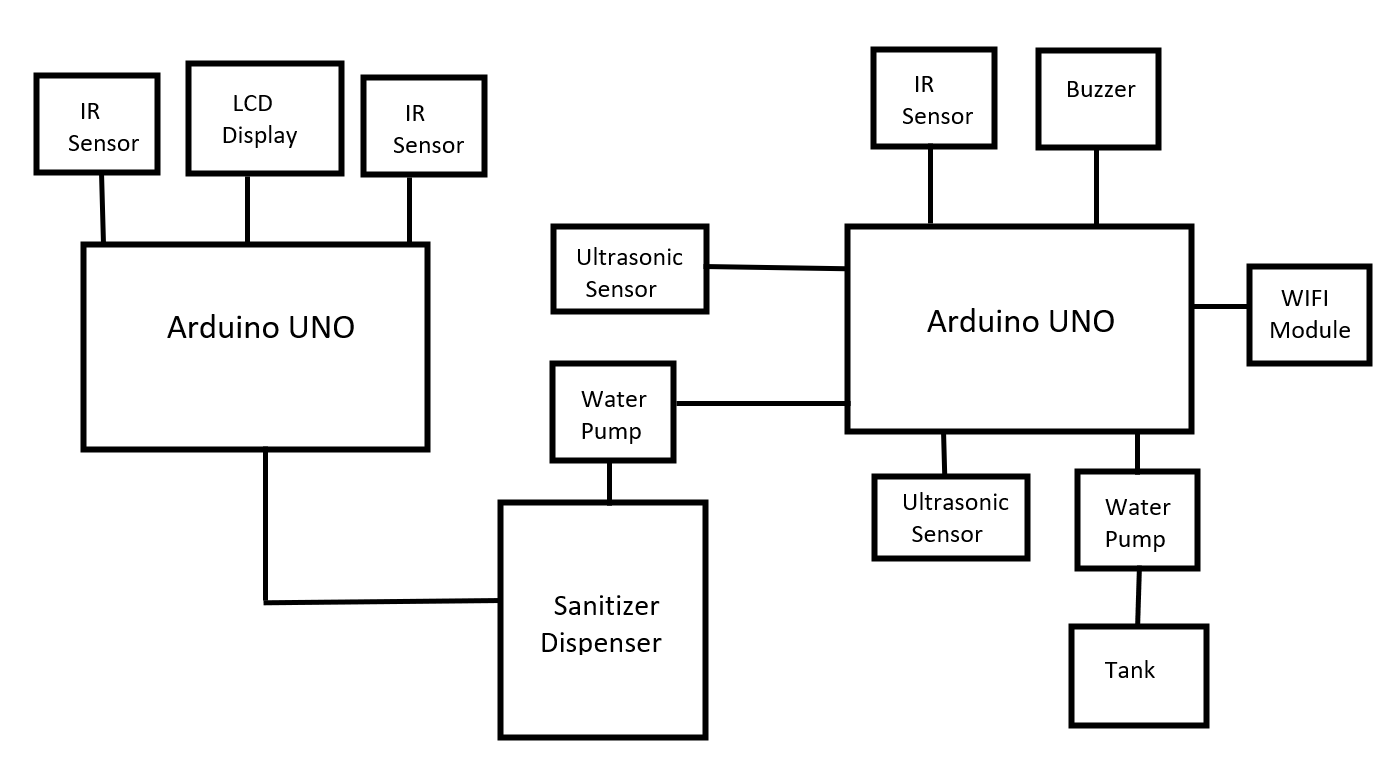
\includegraphics[width=150mm,scale=1]{block}
	\caption{Block Diagram}
	\label{Block Diagram}
	\end{figure}
  \vspace{0.5cm}
  
  \hspace{0.5cm} In this project we have used two Arduinos. One is for Bidirectional visitor counter and other for dispenser and automatic tank filling system. At first Arduino 2 IR sensors are connected for counting number of people entering and leaving premises. At same LCD is connected for display counting. At second Arduino 2 water pumps and 2 ultrasonic sensors are connected. One is for dispense sanitizer liquid and another is for automatic sanitizer tank filling. At this Arduino IR sensor and Buzzer is connected for alert system and WIFI module is connected for sending Alert SMS.

  
 